\chapter{Classical and quantum integrability\label{app:int}}
\thispagestyle{chapterBeginStyle}

\paragraph{Classical integrability}Before jumping head first into the quantum realm, it is perhaps valuable the state
the problem of classical integrability, and the results therein.
We consider this topic in the spirit of the classical discussion
of Liouville and Arnold as presented in a monograph by~\textcite{Gutzwiller1991}.

One usually begins the discussion of classical mechanics with the Lagrangian picture and then
via Legendre transform moves on to the Hamiltonian picture, however we shall skip this
for brevity and take the Hamiltonian picture as a starting point.
A dynamical system at every given time \(t\) is described by its momentum \(p\) and
position \(q\). If we assume our system to have \(n\) degrees of freedoms, then
its state can be specified as a point in a \(2n\)-dimensional space (\(n\) for momenta and
\(n\) for coordinates) called the phase space. Dynamics are governed by a function
of \(H = H(p,q,t)\) called the Hamiltonian, which can be interpreted as the energy,
and the so-called \textit{Hamilton equations of motion}
\begin{equation}
    \dv{p_j}{t} = -\pdv{H}{q_j},\; \; \; \; \dv{q_j}{t} = \pdv{H}{p_j}
    \label{eq:Hamilton equations}
\end{equation} 
Suppose that we have another function on a phase space, say \(F=F(p,q)\), with
a property that its value does not vary in time if we take as \(p\) and \(q\) solutions
of equations~\eqref{eq:Hamilton equations}. This is equivalent to the following condition
\begin{align}
    0 = \dv{}{t}F(p,q) &= \pdv{F}{p} \dv{p}{t} + \pdv{F}{q}\dv{q}{t} \nonumber{}\\
    &= \pdv{H}{p}\pdv{F}{q} - \pdv{H}{q}\pdv{F}{p} = \poissonbracket{H}{F}
\end{align}
where \(\poissonbracket{\bullet }{\bullet }\) is the Poisson bracket.
Vanishing of Poisson bracket with Hamiltonian is a necessary condition for \(F\)
to be called an \textit{integral of motion}. This property has a nice geometric interpretation.
On the one hand, the vector field \(\left(-\pdv*{H}{q},\pdv*{H}{p}\right)\) in a phase space is
tangent to surface \(F(p,q) = const\). On the other hand, the vector field 
\(\left(-\pdv*{F}{q},\pdv*{F}{p}\right)\) is tangent to the energy surface \(H(p,q) = E\).
The trajectory of a dynamical system in a phase space is then located in the intersection
of these two surfaces.
Let us now imagine that we have a set \(\set{F_i}_{i=1,\ldots,k}\) of such conserved
quantities that are functionally independent (no function from this set can be expressed
as a function of other functions from this set). It is not yet sufficient to enable us to solve
the equations of motion. The integrals of motion must also be in \textit{involution},
which means that for any \(F_i,F_j\in\set{F_i}_{i=1,\ldots,k}\) we have
\(\poissonbracket{F_i}{F_j} = 0\). Existence of \(k\) integrals of motion restricts
the dynamics of the system to a \((2n-k)\)-dimensional subspace of the phase space, whereas the fact
that they are in involution guarantees that this subspace has a simple internal structure.
If there are at least \(n\) such conserved quantities, then a famous theorem by
Liouville holds, which states a system with \(n\) degrees of freedom with
\(n\) integrals of motion is integrable by quadratures.
Then, there exists such a canonical transformation \((p,q)\to (F,\Theta)\), to the
so-called angle-action variables, that \(H(p,q) = H(F)\) and the equations
of motions are solved by \(F_j(t) = F_j^0\) and \({\Theta(t)}_j = \Omega_j t + \Theta_j(0)\)~\autocite{arnold2013mathematical}.
Moreover, it was proven with the help of topology that this restricted subspace
has a shape of an \(n\)-dimensional torus, called the \textit{invariant torus}. In
general different initial conditions correspond to different invariant tori.
Therefore, we see that integrability in classical mechanics has a very precise 
definition --- differential equations governing time evolution can be solved explicitly
with the help of action-angle variables. Then, the solutions to equations~\ref{eq:Hamilton equations}
for integrable of motions exhibit periodic dynamics constrained to some invariant torus.
On the other hand, solutions for nonintegrable systems, given sufficient time, explore the whole
phase space.

\paragraph{KAM theorem}Before we leave the classical world, let us ponder upon one more question.
What happens to a classical integrable system under small perturbations? More precisely,
how does the breakdown of invariant tori look like? The answer to this question lies
within the remarkable KAM theorem, which was proven by a joint effort
of~\textcite{Kolmogorov1954,Moser1962,Arnold1963}. For
a system with a finite number of degrees of freedom, it specifies, under some assumptions,
that majority of the invariant tori that occupy\footnote{The more technical term is
\textit{foliate}.} the phase space survive the influence of small perturbations. This entails
the possibility of coexistence between chaos and regularity. Eventually, as perturbation grows,
chaotic regions fill the phase space completely~\autocite{DAlessio2016}. We end this part
with a quote from Arnold's book~\autocite{arnold2013mathematical} about the KAM theorem.
\begin{quotation}
   \textit{ If an unperturbed system is nondegenerate, then for sufficiently
small conservative Hamiltonian perturbations, most non-resonant invariant
tori do not vanish, but are only slightly deformed, so that in the phase space
of the perturbed system, too, there are invariant tori densely filled with phase
curves winding around them conditionally-periodically, with a number of
independent frequencies equal to the number of degrees of freedom.
These invariant tori form a majority in the sense that the measure of the
complement of their union is small when the perturbation is small.}
\end{quotation}
\paragraph{Quantum integrability} After learning about classical integrability, which
is a very mature subject, one may be surprised that the notion of quantum integrability 
is still vigorously debated among scientists. A conclusive answer to the question
`what does it mean for a quantum system to be integrable?' is yet to be found.
In this paragraph, we outline the possible solutions following the reviews
by~\textcite{Caux2011,Yuzbashyan2013}.

First contrasting difference between classical and quantum mechanics is how we count
degrees of freedom. In the former, it corresponds to the number of pairs of conjugate variables
necessary to specify a point in a phase space, each variable admitting a continuum of 
possible values. In the latter, Heisenberg Uncertainty Principle prevents from 
constructing a quantum equivalent of a classical phase space. Furthermore, allowed energy
levels very often constitute a discrete set and thus we can employ finite-dimensional
Hilbert spaces with the dimensionality being the number of degrees of freedom.
This alone prevents us from a straightforward application of classical integrability to quantum
mechanics. Nonetheless, we can try in the spirit of Liouville integrability, consider
a system to be integrable if it possesses a maximal set of conserved quantities 
(operators commuting with a Hamiltonian) of cardinality
equal to the dimension of Hilbert space. Unfortunately, this simple criterion fails immediately,
because by the spectral theorem, Hermitian Hamiltonians can be diagonalized and such
maximal set can be built from projectors on its eigenstates i.e. \(Q_{n} = \ketbra{n}{n}\).
Therefore every system could be called integrable, even though the existence of these projector
operators do not prevent thermalization of physical observables~\autocite{DAlessio2016}.
Shortcomings of this definition can be remedied by requiring the conserved quantities
to be local (or, as recently discovered, quasilocal), that is acting in a nontrivial way
only on some subspace of Hilbert space. As the projection operators are in general very nonlocal,
they are rejected by this constraint. Moreover, we require the number of (quasi)local conserved
charges to be extensive, that is, scaling with the system size. This allows for 
separation between integrable systems and nonintegrable ones, where this quantity is nonextensive.
As mentioned in the Introduction, this definition is sufficient for considerations in this
thesis.

For informational purposes, we shall now list some other possible approaches to the problem at
hand. Mathematical physicists like to say that a system is integrable if it is exactly
solvable, that means a full set of eigenstates can be constructed explicitly. A variety
of techniques can be used to achieve that, for example, Fourier transform for
noninteracting models, and quantum inverse scattering method for one dimensional 
models~\autocite{Faddeev1996,Korepin1993,Ilievski2014}. There are also approaches
to integrability based on non-diffractive scattering (as it leads directly 
to non-ergodicity)~\autocite{Sutherland2004}, or eigenstate entanglement entropy~\autocite{ydzba2020}.
Last but not least, an interesting viewpoint originates from the Berry-Tabor conjecture~\autocite{Berry1977} about the
distribution of energy levels spacings in quantum systems with integrable classical counterparts.
We can take a set of normalized energies~\(\set{e_i}\) with mean spacing equal to unity,
and define \(s_i = e_{i+1}-e_i\), for which we are looking for an universal probability
distribution \(P(s)\) such that for a random choice of \(i\), probability of having
\(s \leq s_i \leq s+\mathrm{d}s\) is \(P(s)\mathrm{ds}\). It was shown to be a Poisson
distribution~\autocite{Ott2002}
\begin{equation}
    P(s) = \exp(-s)
\end{equation}
This result holds also for most integrable systems without the classical limit, but it can fail,
usually due to extra symmetries of Hamiltonian and the resulting degeneracies~\autocite{DAlessio2016}.
Conversely, in chaotic systems Random Matrix Theory predicts emergence of the so-called Wigner-Dyson
statistic. If we consider \(2\cross 2\) Hamiltonians with entries being random numbers from suitable
Gaussian distribution, the energy level spacing distribution is of the form~\autocite{DAlessio2016}
\begin{equation}
    P(s) = A_{\beta} \omega^{\beta} \exp\left[-B_{\beta} \omega^2\right]
\end{equation}
where \(\beta = 1\) if time-reversal symmetry is present and \(\beta = 2\) otherwise.
Constants \(A_{\beta}\) and \(B_{\beta}\) can be fixed by normalization and setting the mean energy level
spacing. Remarkably, one can generalize this result to larger matrices by drawing
them from a suitable Gaussian distribution~\autocite{Alhassid2000}
\begin{equation}
    P(H) \propto \exp\left[-\frac{\beta}{2a^2}\tr\left(H^2\right)\right] =
    \exp\left[-\frac{\beta}{2a^2}\sum_{ij} H_{ij}H_{ji}\right]
    \label{eq:GOE}
\end{equation}
As previously, \(\beta = 1\) for systems with time-reversal invariance, that is
\(H_{ij}\in \RR{}\) and \(H_{ij} = H_{ji}\), whereas \(\beta = 2\) for systems without it,
that is \(H_{ij} \in \CC{}\) and \(H_{ij} = H_{ji}^{\ast}\). In the former case we have
the so-called Gaussian Orthogonal Ensemble (GOE) and in the latter Gaussian Unitary Ensemble (GUE).
As matrices from either GOE or GUE must be invariant under orthogonal and unitary transformation
respectively, the equation~\eqref{eq:GOE} is quite natural, as \(\tr\left(H^2\right)\) is such
invariant~\autocite{DAlessio2016}. A comparison between Poisson and GOE distributions
is shown in Figure~\ref{fig:spacing}. Another interesting difference between integrability and
chaos becomes visible, namely, the repulsion of energy levels, manifested as a vanishing probability
for \(s=0\) in GOE.\@ One could take this as a definition of integrability, however it is probably
more desirable to consider this as a consequence rather than a definition.
\begin{figure}[htbp]
    \centering
    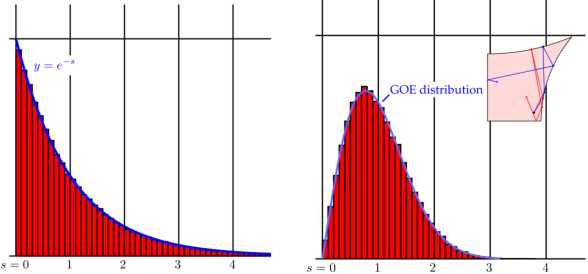
\includegraphics[width=1.0\textwidth,trim={0.03cm 0.03cm 0.03cm 0.03cm},clip]{Figures/spacing.pdf}
    \caption{(Left panel) Distribution of 250000 single-particle level spacings in an integrable system
    --- rectangular box with fine-tuned sides. (Right panel) Distribution of 50000 single-particle
    level spacings in an nonintegrable system shown in the inset. Sourced from~\autocite{DAlessio2016,Rudnick2008}.
     }\label{fig:spacing}
\end{figure}

As in classical mechanics, one may ask a question about the fate of an integrable system
under influence of a weak perturbation. Thus far, we do not have a conclusive answer to this
question, at least not in a form that would be analogous to the KAM theorem. There are results
that show the existence of residual quasiconserved quantities, thus hinting towards a
quantum KAM theorem~\autocite{Brandino2015}. However, it has been also reported that
arbitrarily small perturbations in thermodynamic limit lead to quantum chaos and restoring
of generic (dissipative) dynamics~\autocite{LeBlond2021}. Therefore, as of now, the question of behavior
on the border between integrable and chaotic regimes remains an open problem.